\documentclass[10pt]{article}
\usepackage{icmlko}

\icmlmeta{IP 파운데이션 월드모델}{300}{축은 큰 도메인만 섬긴다}{채택 검사 ③ 을 판 전체에 처음 돌렸다 --- 잴 수 있는 백 자리 중 새로운 것이 서른여섯이고 열한 도메인 중 다섯은 하나도 없다}

\begin{document}

\twocolumn[
\icmlheader

\begin{abstract}
노트 299가 검사 ③(기존 축과의 겹침)을 축 하나에 돌려 ``0 에는 두 가지 뜻이
있다''를 갈랐다. 자동으로 돌게 만들고(\texttt{lab/overlap.py}, 청력과 같이
\textbf{거부권이 아니라 이름표}) \textbf{판 전체에 처음 돌렸다.} 도메인
$\times$ 축 \textbf{184자리} 중 84는 관측 학습행이 30 미만이라 못 재고,
잴 수 있는 \textbf{100자리}가 이렇게 갈린다 --- \textbf{새롭다 36 · 이미
있다 17 · 안 오른다 47}. \textbf{절반 가까이가 아무 정보도 안 나른다.}
그리고 무늬가 도메인별로 갈린다: 웹툰 11 · 애니 9 · 게임 7 이 서른여섯의
\textbf{4분의 3}을 가져가고, \textbf{도서 · 펀딩 · 시장팝업 · 팝업 · 아이돌
다섯은 새로운 축이 0 이다}(아이돌만 2). 검색 · 달력 · 위키 · 태그 열세 축을
쌓아 온 것이 \textbf{큰 도메인만 섬기고 있었다.} 노트 279가 ``판 $\rho$ 는
정식화가 갈리는 자리를 구조적으로 못 본다''고 한 것의 \emph{축 쪽} 짝이다.
그리고 셋째 무늬 --- \textbf{같은 축이 도메인마다 다른 일을 한다.}
\texttt{wiki\_level} 은 세계애니 · 애니 · 웹툰에서 새롭고, 게임 · 만화에서는
\emph{이미 있고}, 모바일에서는 \emph{안 오른다}. 공유 축이라는 이름이 축의
\emph{자리}는 공유하지만 \emph{역할}은 공유하지 않는다.
\end{abstract}
]

\section{검사 ③ 을 자동으로 돌게 만들었다}

노트 239 · 285가 정한 축 채택 검사 셋 중 ③(기존 축과의 겹침)이 거의 안
돌아갔다 --- ① 이 떨어지면 거기서 끝냈고 ① 이 통과하면 곧장 유보 수를 봤다.
노트 299가 축 하나(\texttt{mkt\_cat})에 돌려서 \textbf{0 의 두 가지 뜻}을
갈랐다.

\begin{center}\footnotesize
\begin{tabular}{ll}
\hline
0 의 뜻 & 판정 \\
\hline
\textbf{안 오른다} --- 정보가 없다 & ① 이 떨어진다 \\
\textbf{이미 있다} --- 판이 갖고 있다 & ① 통과 · ③ 떨어짐 \\
\textbf{새롭다} & ① ③ 둘 다 통과 \\
\hline
\end{tabular}
\end{center}

\texttt{lab/overlap.py} 가 그 자리다. 학습 구간에서만 셈하고(노트 285),
공유 축 다섯을 \textbf{값 $+$ 관측 표시자}로 능형에 태워 잔차를 낸 뒤 축을
다시 묻는다 --- \texttt{forms.\_design} 이 쓰는 것과 같은 재료여야 ``판이
이미 갖고 있나''를 묻는 것이 된다. \textbf{승격은 안 막는다}(노트 278$\sim$280
규약, \texttt{hearing.py} 와 같다).

\section{판 전체에 돌렸다}

\begin{figure*}[t]
\centering
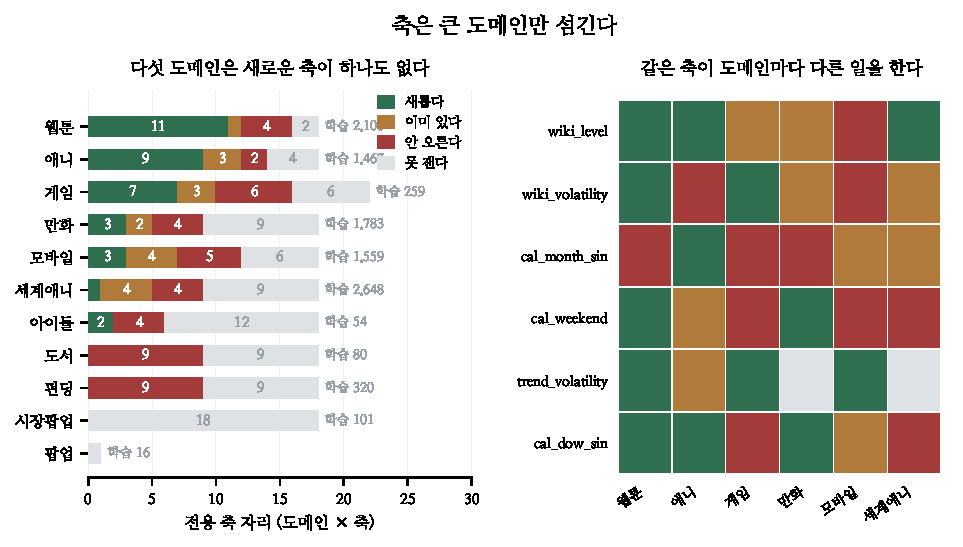
\includegraphics[width=\textwidth]{figs/serve.pdf}
\caption{왼쪽 --- 도메인마다 전용 축 자리의 판정. 오른쪽 --- 같은 축의
도메인별 판정(초록 새롭다 · 주황 이미 있다 · 빨강 안 오른다 · 회색 못 잰다).}
\end{figure*}

\begin{center}\footnotesize
\begin{tabular}{lrrrrr}
\hline
도메인 & 자리 & 새롭다 & 이미 & 안 오름 & 못 잼 \\
\hline
웹툰 & 18 & \textbf{11} & 1 & 4 & 2 \\
애니 & 18 & \textbf{9} & 3 & 2 & 4 \\
게임 & 22 & \textbf{7} & 3 & 6 & 6 \\
만화 & 18 & 3 & 2 & 4 & 9 \\
모바일 & 18 & 3 & 4 & 5 & 6 \\
세계애니 & 18 & 1 & 4 & 4 & 9 \\
아이돌 & 18 & 2 & 0 & 4 & 12 \\
도서 & 18 & \textbf{0} & 0 & 9 & 9 \\
펀딩 & 18 & \textbf{0} & 0 & 9 & 9 \\
시장팝업 & 18 & \textbf{0} & 0 & 0 & 18 \\
팝업 & 1 & \textbf{0} & 0 & 0 & 1 \\
\hline
\textbf{합} & 184 & \textbf{36} & \textbf{17} & \textbf{47} & 84 \\
\hline
\end{tabular}
\end{center}

\paragraph{① 절반 가까이가 빈 열이다} 잴 수 있는 100자리 중 \textbf{47이
``안 오른다''}다 --- 그 도메인에서 그 축이 라벨과 아무 관계가 없다.
17은 ``이미 있다''. \textbf{새로운 것은 36\%뿐이다.}

\paragraph{② 서른여섯 중 스물일곱이 세 도메인 것이다} 웹툰 11 · 애니 9 ·
게임 7 --- \textbf{4분의 3}이다. 그리고

\begin{center}\small
\textbf{도서 · 펀딩 · 시장팝업 · 팝업}에 새로운 축이 \textbf{0개}
\end{center}

다(아이돌은 2). 검색 · 달력 · 위키 · 태그 열세 축을 여러 노트에 걸쳐 쌓아
왔는데 \textbf{그 다섯 도메인에는 아무것도 안 준 것이다.} 시장팝업과 팝업은
아예 전부 ``못 잰다'' --- 그 축들이 관측된 학습행이 30 미만이다.

\paragraph{③ 같은 축이 도메인마다 다른 일을 한다}

\begin{center}\footnotesize
\begin{tabular}{l}
\hline
\texttt{wiki\_level} \\
\quad 세계애니·애니·웹툰 \textbf{새롭다} \\
\quad 게임·만화 \emph{이미 있다} · 모바일 \emph{안 오른다} \\
\hline
\texttt{trend\_volatility} \\
\quad 게임·모바일·웹툰 \textbf{새롭다} \\
\quad 애니 \emph{이미 있다} · 도서·펀딩 \emph{안 오른다} \\
\hline
\texttt{cal\_month\_sin} \\
\quad 애니 \textbf{새롭다} · 모바일·세계애니 \emph{이미 있다} \\
\quad 나머지 여섯 \emph{안 오른다} \\
\hline
\end{tabular}
\end{center}

\textbf{공유 축이라는 이름이 자리는 공유하지만 역할은 공유하지 않는다.}
같은 열이 한 도메인에서는 새 정보이고 다른 도메인에서는 \texttt{target\_
breadth} 가 이미 말한 것이고 또 다른 도메인에서는 잡음이다.

\section{그래서 무엇이 달라지나}

\paragraph{쌓기의 수익이 어디로 갔는지 처음 보인다} 이 실험실은 축을 쌓아
왔고 판 $\rho$ 는 올랐다. 그런데 판 $\rho$ 는 채점 표본 수로 가중하므로
\textbf{웹툰 26.6\% $+$ 애니 22.7\%} 로 절반 가까이가 두 도메인이다(노트 279).
축의 새로움도 같은 두 도메인에 몰려 있다. \textbf{같은 편향이 지표와 자료
양쪽에 있다.}

\paragraph{그리고 노트 296 · 297과 붙는다} 못 재는 84자리는 관측 학습행이
30 미만이라 검사가 안 서는 자리인데, 노트 296이 \textbf{청력 문턱 아래의
행은 사라지는 게 아니라 잡음이 된다}는 것을 봤다. \textbf{못 잰다는 것이
안 들어간다는 뜻이 아니다} --- 그 열들은 지금도 모형에 들어가고 있다.

\begin{center}\small
\begin{tabular}{ll}
\hline
자리 & 지금 하는 일 \\
\hline
새롭다 36 & 정보를 나른다 \\
이미 있다 17 & 같은 말을 두 번 \\
안 오른다 47 & \textbf{잡음} \\
못 잰다 84 & \textbf{모름 --- 그런데 들어간다} \\
\hline
\end{tabular}
\end{center}

\paragraph{남은 것}
\begin{center}\small
\begin{tabular}{ll}
\hline
갈래 & 왜 \\
\hline
안 오르는 47 을 빼면 & 노트 292가 잡음이 해친다고 \\
작은 다섯을 위한 축 & 지금 축은 그쪽에 안 닿는다 \\
겹침을 실행 기록에 & 청력처럼 \texttt{cfg} 에 \\
위약 팔 & 신호가 내용이냐 모양이냐 \\
\hline
\end{tabular}
\end{center}

\paragraph{규약} \textbf{축을 더하기 전에 그 축이 누구에게 닿는지 세라.}
검색 · 달력 · 위키 · 태그를 쌓을 때마다 판 $\rho$ 로만 확인했고, 판 $\rho$ 는
큰 도메인 것이다. \textbf{``판이 올랐다''는 ``모두에게 좋아졌다''가 아니다}
--- 백 자리 중 서른여섯이 새롭고 그 서른여섯의 4분의 3이 세 도메인 것이다.
그리고 \textbf{한 축의 판정은 도메인마다 따로 물어야 한다} --- 같은 열이
어디서는 정보이고 어디서는 중복이고 어디서는 잡음이다.

\end{document}
